\section{Recommender Systems}

\subsection{Introduzione}

Un sistema di raccomandazione (Recommender System) \cite{RecommenderOverview} è un sistema software progettato per suggerire all'utente elementi di interesse, come ad esempio prodotti, servizi, informazioni o contenuti multimediali, in base alle preferenze e ai comportamenti passati dell'utente. I sistemi di raccomandazione sono ampiamente utilizzati in diversi contesti, come ad esempio il commercio elettronico, i social network, i servizi di streaming multimediale e le piattaforme di ricerca e informazione. I sistemi di raccomandazione sono utili per migliorare l'esperienza dell'utente, aumentare la soddisfazione e la fidelizzazione del cliente, e favorire la scoperta di nuovi contenuti e opportunità.
Questi sistemi sono basati su algoritmi di apprendimento automatico e intelligenza artificiale, che analizzano i dati relativi alle preferenze e ai comportamenti degli utenti, e generano raccomandazioni personalizzate in base a tali informazioni.\\

\begin{figure}[h!]
    \centering
    \begin{minipage}{0.2\textwidth}
        \centering
        
\includegraphics[width=\textwidth]{images/netflix.png}
    \end{minipage}\hfill
    \begin{minipage}{0.2\textwidth}
        \centering
        
\includegraphics[width=\textwidth]{images/amazon.png}
    \end{minipage}\hfill
    \begin{minipage}{0.2\textwidth}
        \centering
        
\includegraphics[width=\textwidth]{images/spotify.png}
    \end{minipage}\hfill
    \begin{minipage}{0.2\textwidth}
        \centering
        
\includegraphics[width=\textwidth]{images/tiktok.png}
    \end{minipage}
    \caption{Alcuni famose piattaforme che utilizzano sistemi di raccomandazione}
\end{figure}


\noindent I sistemi di raccomandazione possono essere di diversi tipi, a seconda della tecnica utilizzata per generare le raccomandazioni.
\begin{itemize}
    \item \textbf{Collaborative filtering} \cite{CFRS}: generano raccomandazioni basandosi sulle valutazioni degli utenti per gli item
    \item \textbf{Content-based} \cite{Lops2011}: generano raccomandazioni basandosi sul contenuto degli item e sulle preferenze dell'utente
    \item \textbf{Knowledge-aware} \cite{KnowledgeBased}: generano raccomandazioni basandosi su conoscenza semantica, rappresentata mediante i knowledge-graph
    \item \textbf{Approci ibridi}: combinano le tecniche precedenti
\end{itemize}



\begin{table}[H]
    \centering
    \footnotesize
    \setlength\tabcolsep{0pt}
    \begin{tabularx}{\textwidth}{|X|X|}
        \hline
        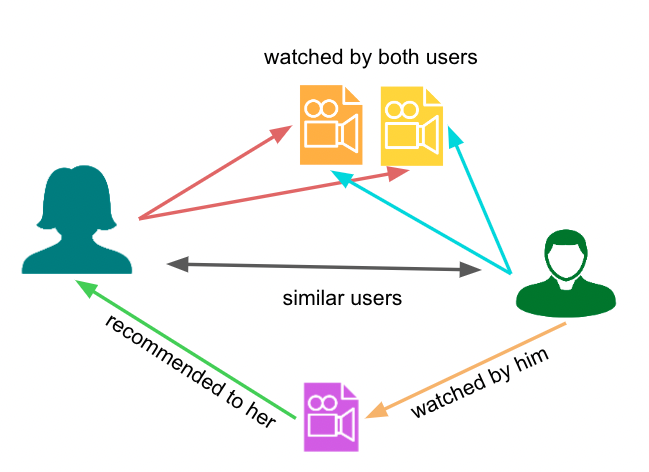
\includegraphics[width=\linewidth, trim=0 0 0 0]{images/cfRecSys.png} &
        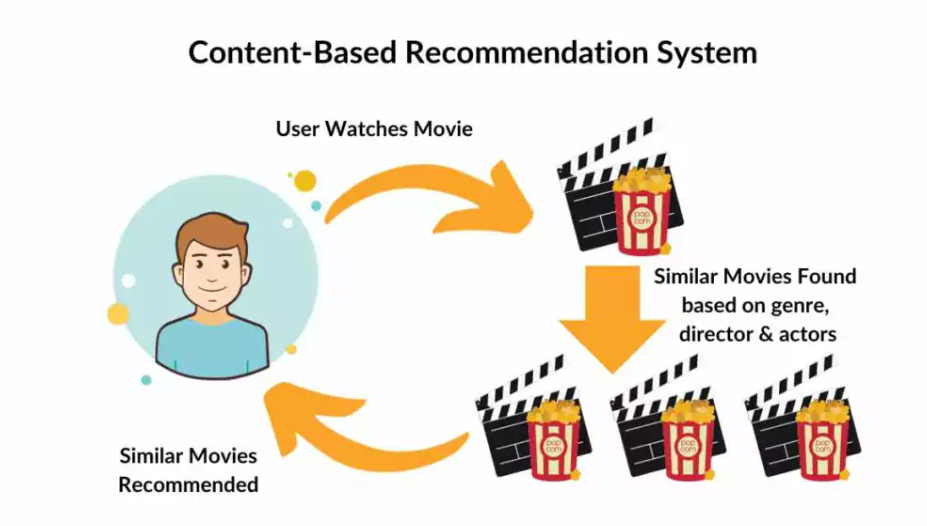
\includegraphics[width=\linewidth, trim=0 0 0 0]{images/contentbased.png} \\
        \hline
        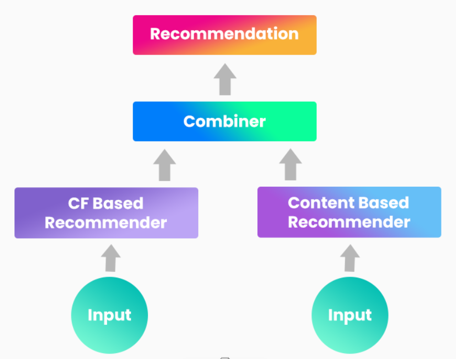
\includegraphics[width=\linewidth, trim=0 0 0 0]{images/hybridRecSys.png} &
        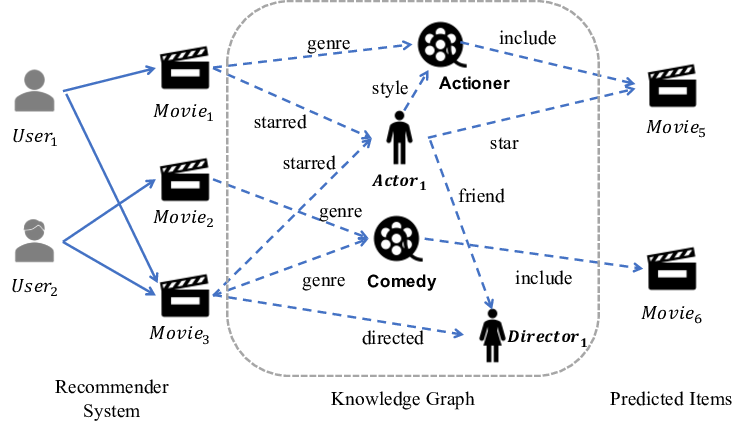
\includegraphics[width=\linewidth, trim=0 0 0 0]{images/knowledge.png} \\
        \hline
    \end{tabularx}
    \caption{Tipi di Recommender Systems}
\end{table}


\noindent Per valutare le prestazioni di un sistema di raccomandazione si possono utilizzare diverse metriche che è possibile riassumere nelle seguenti categorie:
\begin{itemize}    
    \item \textbf{Classification metrics}: queste metriche valutano la capacità del sistema di classificare correttamente gli elementi in base alle preferenze dell'utente. Alcune delle metriche più comuni sono l'accuracy, la precision, il recall e l'F1-score.

    \item \textbf{Accuracy metrics}: queste metriche valutano la precisione e l'accuratezza delle raccomandazioni generate dal sistema. Alcune delle metriche più comuni sono l'RMSE (Root Mean Squared Error) e il MAE (Mean Absolute Error).
    \item \textbf{Ranking metrics}: queste metriche valutano la qualità dell'ordinamento delle raccomandazioni generate dal sistema. Alcune delle metriche più comuni sono il coefficiente di correlazione di Kendall Tau, il coefficiente di correlazione di Spearman, l'NDCG (Normalized Discounted Cumulative Gain).
    \item \textbf{Diversity metrics}: queste metriche valutano la diversità delle raccomandazioni generate dal sistema. Alcune delle metriche più comuni sono la diversità delle raccomandazioni e la novità delle raccomandazioni.
    \item \textbf{Coverage metrics}: queste metriche valutano la copertura degli elementi raccomandati dal sistema.
\end{itemize}    

\noindent Alcuni tipici problemi che si possono incontrare nella progettazione e nell'implementazione di un sistema di raccomandazione sono:
\begin{itemize}
    \item \textbf{Cold start problem} \cite{ColdStart}: il problema del cold start si verifica quando un nuovo utente o un nuovo elemento si registra nel sistema e non ci sono dati sufficienti per generare raccomandazioni personalizzate.
    \item \textbf{Data sparsity problem} \cite{DataSparsity}: nella maggior parte delle reali applicazioni il numero di item è molto maggiore del numero di item valutati da ciascun utente. Questo porta a una matrice di valutazioni molto sparsa, che rende difficile la generazione di raccomandazioni accurate
    \item \textbf{Vulnerabilità agli attacchi} \cite{Attacchi} : i sistemi di raccomandazione possono essere vulnerabili a diversi tipi di attacchi, come ad esempio le recensioni fake (tipico problema degli e-commerce)
\end{itemize}

\subsection{Collaborative Filtering}
I sistemi di raccomandazione collaborative filtering generano raccomandazioni/filtrano i contenuti basandosi sull' "opinione" di altri utenti.\\ Con il termine utente ci si riferisce a qualsiasi individuo che inserisca delle valutazioni per gli item presenti nel sistema. \\ Gli item sono gli oggetti che vengono raccomandati agli utenti (es. film, libri, prodotti, etc.).\\
L'idea alla base del collaborative filtering è creare una matrice di valutazioni utente-item, in cui ogni cella della matrice rappresenta la valutazione di un utente per un item.\\ Le valutazioni sono in genere numeriche, e possono essere espresse in termini di rating (es. da 1 a 5 stelle) o di preferenze (es. like/dislike).\\
Esistono principalmente due tipi di collaborative filtering:
\begin{itemize}
    \item \textbf{User-based collaborative filtering}: in questo approccio, le raccomandazioni vengono generate confrontando le preferenze dell'utente con quelle degli altri utenti. In particolare, si calcola la similarità tra l'utente target e gli altri utenti, e si generano raccomandazioni basate sulle preferenze degli utenti più simili all'utente target. Due utenti sono ritenuti simili se hanno uno stile di valutazione simile per gli item (cioè valutano gli stessi item in modo simile)
    \item \textbf{Item-based collaborative filtering}: in questo approccio, le raccomandazioni vengono generate confrontando le preferenze degli utenti per gli item. In particolare, si calcola la similarità tra gli item, e si generano raccomandazioni basate sugli item più simili a quelli valutati positivamente dall'utente target. Due item sono ritenuti simili se vengono valutati in modo simile dagli stessi utenti.
\end{itemize}
I principali vantaggi del collaborative filtering sono la sua semplicità e la sua capacità di generare raccomandazioni personalizzate senza la necessità di dover conoscere le caratteristiche degli item (es. la durata di un film, il genere di un libro, etc.). Tuttavia, il collaborative filtering può soffrire di problemi come il cold start (per un nuovo utente e per un nuovo item), la vulnerabilità agli attacchi come le recensioni fake e la scarsa spiegaibilità delle raccomandazioni generate.\\

%crea un esempio di matrice utente-item
\begin{table}[H]
    \centering
    \begin{tabular}{|c|c|c|c|c|}
        \hline
        & Item 1 & Item 2 & Item 3 & Item 4 \\
        \hline
        User 1 & 5 & 4 & 0 & 0 \\ \hline
        User 2 & 0 & 0 & 3 & 4 \\ \hline
        User 3 & 0 & 0 & 0 & 0 \\ \hline
        User 4 & 0 & 0 & 0 & 0 \\
        \hline
    \end{tabular}
    \caption{Esempio di matrice utente-item}
\end{table}


\subsection{Content-based}
I sistemi di raccomandazione content-based generano raccomandazioni basate sul contenuto degli elementi e sulle preferenze dell'utente. Questi sistemi analizzano le caratteristiche degli elementi e le preferenze dell'utente, e generano raccomandazioni in base alla somiglianza tra gli elementi e le preferenze dell'utente. Per preferenze dell'utente si intendono le caratteristiche degli elementi che l'utente ha valutato in passato.
Un sistema di raccomandazione content-based è composto da tre componenti principali:
\begin{itemize}
    \item \textbf{Profile learner}: Questa componente colleziona i dati relativi alle preferenze dell'utente e cerca di generalizzarle per creare un profilo dell'utente. Spesso questa generalizzazione avviene mediante tecniche di apprendimento automatico.
    \item \textbf{Content analyzer}: Questa componente ha come scopo quello di estrarre le caratteristiche degli item. Quando le descrizioni non sono strutturate (es. testo) è necessaria una fase di pre-processing per estrarre le caratteristiche rilevanti.
    \item \textbf{Filtering Component}: Questa componente ha come scopo quello di generare raccomandazioni personalizzate in base al profilo dell'utente e alle caratteristiche degli item. In particolare, si calcola la somiglianza tra il profilo dell'utente e le caratteristiche degli item, e si generano raccomandazioni basate su questa somiglianza.
\end{itemize}
I principali vantaggi sono l'indipendenza dal comportamento degli altri utenti e la capacità di generare raccomandazioni personalizzate anche per nuovi item. Inoltre c'è una maggiore spiegabilità delle raccomandazioni generate. Tuttavia, i sistemi di raccomandazione content-based possono soffrire di problemi come la scarsa diversità delle raccomandazioni e la difficoltà di estrarre le caratteristiche rilevanti degli item. Rimane comunque il problema di cold-start per un nuovo utente.
\subsection{Knowledge-aware}
I sistemi di raccomandazione knowledge-aware generano raccomandazioni basandosi su conoscenza semantica, rappresentata mediante i knowledge-graph. I knowledge-graph sono grafi in cui i nodi rappresentano concetti e le relazioni tra i concetti, e gli archi rappresentano le relazioni tra i concetti. I sistemi di raccomandazione knowledge-aware utilizzano i knowledge-graph per rappresentare le caratteristiche degli item e le preferenze dell'utente, e generare raccomandazioni basate su questa rappresentazione. In particolare, si utilizzano tecniche di reasoning per inferire nuove conoscenze a partire dalle conoscenze esistenti, e generare raccomandazioni basate su queste nuove conoscenze. I principali vantaggi dei sistemi di raccomandazione knowledge-aware l'assenza del problema di cold-start. Tuttavia, i sistemi di raccomandazione knowledge-aware possono soffrire di problemi come la scarsa spiegabilità delle raccomandazioni generate e la difficoltà di rappresentare la conoscenza semantica in modo accurato e completo. Inoltre, i sistemi di raccomandazione knowledge-aware possono richiedere una quantità significativa di risorse computazionali per generare raccomandazioni accurate e rilevanti.\\

\subsection{Modelli di raccomandazione a stato dell'arte}
Negli ultimi anni, sono stati proposti diversi modelli di raccomandazione basati su diverse tecniche, che hanno ottenuto risultati molto promettenti in termini di accuratezza e prestazioni. Questi modelli sono chiamati a stato dell'arte (\textbf{SOTA}) per l'implementazione di sistemi di raccomandazione. Alcuni esempi di modelli di raccomandazione a stato dell'arte sono:
\begin{itemize}
    \item \textbf{ItemKNN} \cite{ItemKNN}: ItemKNN è un modello di raccomandazione basato su collaborative filtering item-based. In particolare, ItemKNN calcola la similarità tra gli item e genera raccomandazioni basate sugli item più simili a quelli valutati positivamente dall'utente target.
    \item \textbf{BPR} \cite{BPR}: BPR (Bayesian Personalized Ranking) è un modello di raccomandazione basato su collaborative filtering user-based. In particolare, BPR calcola la similarità tra gli utenti e genera raccomandazioni basate sugli utenti più simili all'utente target.
    \item \textbf{CFKG} \cite{CFKG}: CFKG è un modello di raccomandazione basato su collaborative filtering e knowledge-aware. In particolare, CFKG utilizza i knowledge-graph per rappresentare le caratteristiche degli item e le preferenze dell'utente, e genera raccomandazioni basate su questa rappresentazione.
    \item \textbf{CKE} \cite{CKE}: CKE (Collaborative Knowledge Embedding) è un modello di raccomandazione basato su collaborative filtering e knowledge-aware. In particolare, CKE utilizza tecniche di embedding per rappresentare le caratteristiche degli item e le preferenze dell'utente, e genera raccomandazioni basate su questa rappresentazione.
    \item \textbf{DMF} \cite{DMF}: DMF (Deep Matrix Factorization) è un modello di raccomandazione basato su deep learning. In particolare, DMF utilizza tecniche di deep learning per apprendere le rappresentazioni latenti degli item e degli utenti, e genera raccomandazioni basate su queste rappresentazioni.
    \item \textbf{KGCN} \cite{KGCN}: KGCN (Knowledge Graph Convolutional Networks) è un modello di raccomandazione basato su deep learning e knowledge-aware. In particolare, KGCN utilizza tecniche di deep learning e convolutional neural networks per apprendere le rappresentazioni degli item e degli utenti a partire dai knowledge-graph, e genera raccomandazioni basate su queste rappresentazioni.
    \item \textbf{KGNNLS} \cite{KGNNLS}: KGNNLS (Knowledge Graph Neural Network with Latent Space) è un modello di raccomandazione basato su deep learning e knowledge-aware. In particolare, KGNNLS utilizza tecniche di deep learning e neural networks per apprendere le rappresentazioni degli item e degli utenti a partire dai knowledge-graph, e genera raccomandazioni basate su queste rappresentazioni.
    \item \textbf{LINE} \cite{LINE}: LINE (Large-scale Information Network Embedding) è un modello di raccomandazione basato su deep learning e knowledge-aware. In particolare, LINE utilizza tecniche di deep learning e neural networks per apprendere le rappresentazioni degli item e degli utenti a partire dai knowledge-graph, e genera raccomandazioni basate su queste rappresentazioni.
    \item \textbf{MultiDAE} \cite{MultiDAE}: MultiDAE è un modello di raccomandazione basato su deep learning. In particolare, MultiDAE utilizza tecniche di deep learning e variational autoencoders per apprendere le rappresentazioni latenti degli item e degli utenti, e genera raccomandazioni basate su queste rappresentazioni.
    \item \textbf{LightGCN} \cite{LightGCN}: LightGCN è un modello di raccomandazione basato su deep learning. In particolare, LightGCN utilizza tecniche di deep learning e graph convolutional networks per apprendere le rappresentazioni latenti degli item e degli utenti, e genera raccomandazioni basate su queste rappresentazioni.
    \item \textbf{NGCF} \cite{NGCF}: NGCF (Neural Graph Collaborative Filtering) è un modello di raccomandazione basato su deep learning. In particolare, NGCF utilizza tecniche di deep learning e graph convolutional networks per apprendere le rappresentazioni latenti degli item e degli utenti, e genera raccomandazioni basate su queste rappresentazioni.
    \item \textbf{DGCF} \cite{DGCF}: DGCF (Dual Graph Collaborative Filtering) è un modello di raccomandazione basato su deep learning. In particolare, DGCF utilizza tecniche di deep learning e graph convolutional networks per apprendere le rappresentazioni latenti degli item e degli utenti, e genera raccomandazioni basate su queste rappresentazioni.
\end{itemize}


\noindent Ovviamente ci sono tanti altri modelli di raccomandazione a stato dell'arte, ma questi sono solo alcuni esempi.\\
I progettisti di Recommender Systems spesso prendono spunto da questi modelli per creare nuovi modelli che possano adattarsi meglio alle esigenze specifiche del problema che si vuole risolvere.\\



\subsection{Recommender Systems e Sustainability}

I sistemi di raccomandazione, così come tutti gli altri modelli di AI, possono essere utilizzati per promuovere la sostenibilità in tutti i suoi punti, ad esempio cercando di adempiere agli obiettivi dell'Agenda 2030 \cite{RecommenderSustainability}.

\noindent In ambito \textit{energia pulita e riduzione delle emissioni} viene suggerito come i sistemi di raccomandazione possano essere utilizzati per promuovere l'adozione di comportamenti sostenibili, ad esempio suggerendo all'utente di utilizzare mezzi di trasporto pubblici o condivisi, di ridurre il consumo di energia elettrica o di acquistare prodotti sostenibili. Inoltre, i sistemi di raccomandazione possono essere utilizzati per promuovere l'adozione di energie rinnovabili e la riduzione delle emissioni di gas serra. In questo caso si parla dunque di sistemi di raccomandazione i quali cercano di promuovere comportamenti sostenibili, ma a loro vola per essere addestrati richiedono grandi quantità di dati e di risorse computazionali, che possono avere un impatto negativo sull'ambiente.

\noindent Una soluzione dunque può essere quella di addestrare i modelli di raccomandazione in modo sostenibile, senza però perdere di performance.


